%------------------------------------------------------------------------------------------------%

\chapter{Theoretical Background}

%------------------------------------------------------------------------------------------------%
This chapter is mainly based on the dissertation of Daniel Köhn (\cite{koehn:11}), who originally has written this manual.
\section{Equations of motion for an elastic medium}\label{elastic_fd_model} 
The propagation of waves in a general elastic medium can be described by a system of coupled linear partial differential equations. They consist of the equations of motion
\EQ{m:1}{\begin{split}
\rm{\rho \frac{\partial v_i}{\partial t}} &\rm{= \frac{\partial \sigma_{ij}}{\partial x_j} + f_i}\\
\end{split}}   
which simply state that the momentum of the medium, the product of density $\rm{\rho}$ and the displacement velocity $\rm{v_i}$, can be changed by surface forces, described by the stress tensor $\rm{\sigma_{ij}}$ or body forces $\rm{f_i}$. These equations describe a general medium, like gas, fluid, solid or plasma. The material specific properties are introduced by additional equations which describe how the medium reacts when a certain force is applied. In the isotropic elastic case this can be described by a linear stress-strain relationship:  
\EQ{m:2}{\begin{split}
\rm{\sigma_{ij}}&\rm{=\lambda \theta \delta_{ij} + 2 \mu \epsilon_{ij}}\\
\rm{\epsilon_{ij}}&\rm{=\frac{1}{2}\biggl(\frac{\partial u_i}{\partial x_j}+\frac{\partial u_j}{\partial x_i}\biggr)}
\end{split}}   
where $\rm{\lambda}$ and $\rm{\mu}$ are the Lam$\rm{\acute{e}}$ parameters, $\rm{\epsilon_{ij}}$ the strain tensor and $\rm{u_i}$ the displacement. Using $\rm{v_i = \frac{\partial u_i}{\partial t}}$, \ER{m:1} and \ER{m:2} can be transformed into a system of second order partial differential equations:
\EQ{2:20}{\begin{split}
\rm{\rho \frac{\partial^2 u_i}{\partial t^2}} &\rm{= \frac{\partial \sigma_{ij}}{\partial x_j} + f_i}\\
\rm{\sigma_{ij}}&\rm{=\lambda \theta \delta_{ij} + 2 \mu \epsilon_{ij}}\\
\rm{\epsilon_{ij}}&\rm{=\frac{1}{2}\biggl(\frac{\partial u_i}{\partial x_j}+\frac{\partial u_j}{\partial x_i}\biggr)}
\end{split}}
This expression is called {\bf{Stress-Displacement}} formulation. Another common form of the elastic equations of motion can be deduced by taking the time derivative of the stress-strain relationship and the strain tensor in Eq. \ER{2:20}. Since the Lam$\acute{\rm e}$ parameters $\rm{\lambda}$ and $\rm{\mu}$ do not depend on time, Eq. \ER{2:20} can be written as:
\EQ{2:20:1}{\begin{split}
\rm{\rho \frac{\partial v_i}{\partial t}} &\rm{= \frac{\partial \sigma_{ij}}{\partial x_j} + f_i}\\
\rm{\frac{\partial \sigma_{ij}}{\partial t}} &\rm{= \lambda \frac{\partial \theta}{\partial t} \delta_{ij} + 2 \mu \frac{\partial \epsilon_{ij}}{\partial t}}\\
\rm{\frac{\partial \epsilon_{ij}}{\partial t}}&\rm{=\frac{1}{2}\biggl(\frac{\partial v_i}{\partial x_j}+\frac{\partial v_j}{\partial x_i}\biggr)}
\end{split}}  
This expression is called {\bf{Stress-Velocity}} formulation. For simple cases \ER{2:20} and \ER{2:20:1} can be solved analytically. More complex problems require numerical solutions. One possible approach for a numerical solution is described in the next section.
\section{Solution of the elastic wave equation by finite differences}\label{elastic_FD_Code}
\subsection{Discretization of the wave equation}
For the numerical solution of the elastic equations of motion, Eqs. \ER{2:20} have to be discretized in time and space on a grid. The
particle velocity $\rm{\mathbf{v}}$, the stresses $\rm{\sigma_{ij}}$, the Lam$\acute{\rm e}$ parameters $\rm{\lambda}$ and $\rm{\mu}$ are calculated and defined at discrete Cartesian coordinates $\rm{x=i\; dh}$, $\rm{y=j\; dh}$ and discrete times $\rm{t=n\; dt}$. 
$\rm{dh}$ denotes the spatial distance between two adjacent grid points and $\rm{dt}$ the difference between two successive time steps. Therefore every grid point is located in the interval  $\rm{i \in N | [1,NX]}$, $\rm{j \in N | [1,NY]}$ and $\rm{n \in N | [1,NT]}$, where
$\rm{NX}$, $\rm{NY}$ and $\rm{NT}$ are the number of discrete spatial grid points and time steps, respectively. Finally the partial derivatives are replaced by {\bf{finite-difference} (FD)} operators. 
Two types of operators can be distinguished, forward and backward operators $\rm{D^+,\;D^-}$. The derivative of a function y with respect to a variable x can be approximated by the following operators:  
\EQ{disc:1}{\begin{split}
\rm{D^+_x y}&\rm{= \frac{y[i+1]-y[i]}{dh} \hspace{1 cm} \text{forward operator}}\\
\rm{D^-_x y}&\rm{= \frac{y[i]-y[i-1]}{dh} \hspace{1 cm} \text{backward operator}}\\
\end{split}}\\
To calculate the spatial derivatives of the wavefield variables at the correct positions, the variables are not placed on the same 
grid points, but staggered by half of the spatial grid point distance (\cite{virieux:86} and \cite{levander:88}). 
\FIG{SSG-Cart.eps} shows the distribution of the material parameters and wavefield variables on the spatial grid. 


\begin{figure}[bh]
\begin{center}
\begin{tikzpicture}[scale=6]

\draw[thick,->] (0,0,0) -- (1.2,0,0) node[anchor=north]{$\rm x$};
\draw[thick,->] (0,0,0) -- (0,-1.2,0) node[anchor=west]{$\rm y$};

\draw (0.5,0,0) -- (0.5,-0.5,0);
\draw (0,-0.5,0) -- (0.5,-0.5,0);

\draw[line width=2pt,color=black] (0.49,-0.51) -- (0.51,-0.51) -- (0.51,-0.49) -- (0.49,-0.49) -- cycle;
\draw[line width=2pt,color=black] (0.49,-0.01) -- (0.51,-0.01) -- (0.50,0.01) -- cycle;
\draw[line width=2pt,color=black] (-0.01,-0.49) -- (0.01,-0.49) -- (0.00,-0.51) -- cycle;

\fill[black] (0,0,0) circle (0.6pt) node [anchor=south]{$\rm (i,j)$} node 
[anchor=north west]{$\rm \sigma_{xx}$, $\sigma_{yy}$};
\fill[black] (0,-0.07,0) node [anchor=north west]{$\rm\rho$, $\lambda$, $\mu$};

\fill (0,-1,0) circle (0.5pt) node [anchor=west]{$\rm (i,j+1)$};
\fill (1,0,0) circle (0.5pt) node [anchor=south]{$\rm (i+1,j)$};

\fill[black] (0.5,0,0)  node [anchor=north 
west]{$\rm v_{x}$, $\rm\rho_x$};
\fill[black] (0,-0.5,0)  node [anchor=north 
west]{$\rm v_{y}$, $\rm\rho_y$};
\fill[black] (0.5,-0.5,0) circle (0.2pt) node [anchor=north 
west]{$\rm\sigma_{xy}$, $\mu_{xy}$};

\fill[black] (0.8,-0.8,0) node [anchor=north 
west]{$\rm\lambda=\rho\left(v_p^2-2v_s^2\right)$};
\fill[black] (0.8,-0.95,0) node [anchor=north west]{$\rm\mu=\rho v_s^2$};

\end{tikzpicture}
\caption{\label{SSG-Cart.eps} Grid geometry for a standard staggered grid (SSG) in Cartesian coordinates as suggested by 
\cite{virieux:86} and \cite{levander:88}.}
\label{fig_cell}
\end{center}
\end{figure}  

% \caption[Staggered Grid]{Cell of the SSG with elastic 
%  modelling parameters. Stress tensor elements 
% $\sigma_{ij}$, seismic velocities $v_i$ and modell 
% parameters $\lambda$, $\mu$ and $\rho$.}
% \end{figure}
 
% \begin{figure}[bh]
% \begin{center}
% 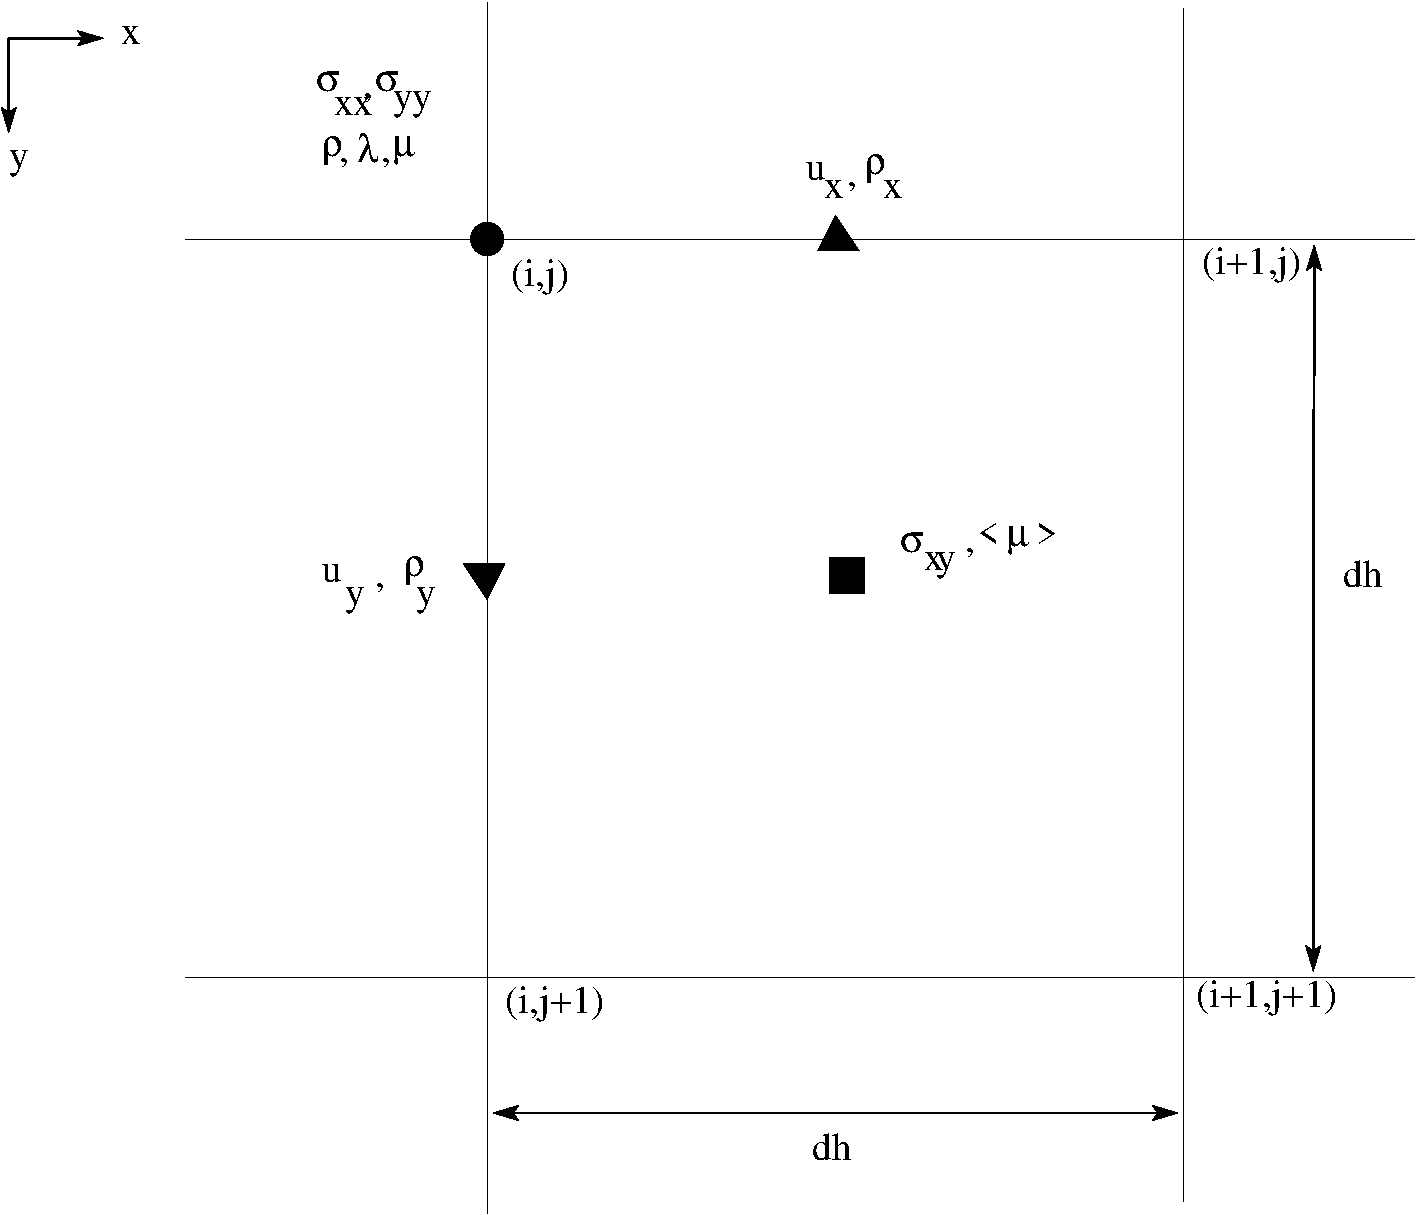
\includegraphics[width=.6\textwidth]{figures/SSG-Cart}
% \caption{\label{SSG-Cart.eps} Grid geometry for a standard staggered grid (SSG) in Cartesian coordinates as suggested by 
% \cite{virieux:86} and \cite{levander:88}.}
% \label{fig_cell}
% \end{center}
% \end{figure}   

To guarantee the stability of the {\bf{standard staggered grid (SSG)}} code, the Lam$\acute{\rm e}$ parameter $\rm{\mu}$ and density $\rm{\rho}$ have to be averaged 
harmonically and arithmetically (\cite{moczo:04}, \cite{bohlen:06}), respectively
\EQ{disc:2}{\begin{split}
\rm{\mu_{xy}[j+\frac{1}{2}][i+\frac{1}{2}]}&\rm{=\biggl[\frac{1}{4}\biggl(\mu^{-1}[j][i]+\mu^{-1}[j][i+1]+\mu^{-1}[j+1][i+1]+\mu^{-1}[j+1][i]\biggr)\biggr]^{-1}}\\ 
\rm{\rho_x[j][i+\frac{1}{2}]}&\rm{=\frac{1}{2}(\rho[j][i+1]+\rho[j][i])}\\
\rm{\rho_y[j+\frac{1}{2}][i]}&\rm{=\frac{1}{2}(\rho[j+1][i]+\rho[j][i])}\\
\end{split}}  
The discretization of the linear stress velocity relationship in \ER{2:20:1} at time step n leads to the following system of equations: % (for simplicity I skip the time index n): 
\EQ{cart_dis:1}{\begin{split}
\rm{v_{xx}[j][i]}&\rm{\approx \frac{v_x[j][i+\frac{1}{2}]-v_x[j][i-\frac{1}{2}]}{dh}}\\ 
\rm{v_{yy}[j][i]}&\rm{\approx \frac{v_y[j+\frac{1}{2}][i]-v_y[j-\frac{1}{2}][i]}{dh}}\\ 
\rm{v_{yx}[j+\frac{1}{2}][i+\frac{1}{2}]}&\rm{\approx \frac{v_y[j+\frac{1}{2}][i+1]-v_y[j+\frac{1}{2}][i]}{dh}}\\ 
\rm{v_{xy}[j+\frac{1}{2}][i+\frac{1}{2}]}&\rm{\approx \frac{v_x[j+1][i+\frac{1}{2}]-v_x[j][i+\frac{1}{2}]}{dh}}\\ 
\rm{\sigma^{n+1}_{xy}[j+\frac{1}{2}][i+\frac{1}{2}]}&\rm{=\sigma^{n}_{xy}[j+\frac{1}{2}][i+\frac{1}{2}] + dt\cdot\mu_{xy}[j+\frac{1}{2}][i+\frac{1}{2}]\biggl(v_{xy}[j+\frac{1}{2}][i+\frac{1}{2}] + v_{yx}[j+\frac{1}{2}][i+\frac{1}{2}]\biggr)}\\ 
\rm{\sigma^{n+1}_{xx}[j][i]}&\rm{= \sigma_{xx}^{n}[j][i] + dt\cdot\lambda[j][i]\cdot \biggl(v_{xx}[j][i] + v_{yy}[j][i] \biggr) + 2 dt\cdot  \mu_{xy}[j][i] \cdot  v_{xx}[j][i]}\\ 
\rm{\sigma^{n+1}_{yy}[j][i]}&\rm{= \sigma_{yy}^{n}[j][i] + dt\cdot\lambda[j][i]\cdot \biggl(v_{xx}[j][i] + v_{yy}[j][i] \biggr) + 2 dt\cdot  \mu_{xy}[j][i] \cdot  v_{yy}[j][i]}\\ 
\end{split}} 
 
The discretization of the momentum equation in \ER{2:20:1} leads to the following system of equations:
\EQ{cart_dis:2}{\begin{split}
\rm{vtt_x^n[j][i+\frac{1}{2}]} &\rm{= \biggl(\sigma_{xx}[j][i+1] - \sigma_{xx}[j][i] + \sigma_{xy}[j+\frac{1}{2}][i] - \sigma_{xy}[j-\frac{1}{2}][i] \biggr)}\\
\rm{vtt_y^n[j+\frac{1}{2}][i]} &\rm{= \biggl(\sigma_{xy}[j][i+\frac{1}{2}] - \sigma_{xy}[j][i-\frac{1}{2}] + \sigma_{yy}[j+1][i] - \sigma_{yy}[j][i] \biggr)}\\ 
\rm{v_x^{n+1}[j][i+\frac{1}{2}]}&\rm{= v_x^{n}[j][i+\frac{1}{2}] + \frac{dt}{dh\cdot \rho_x[j][i+\frac{1}{2}]}\cdot vtt_x^n[j][i+\frac{1}{2}]}\\
\rm{v_y^{n+1}[j+\frac{1}{2}][i]}&\rm{= v_y^{n}[j+\frac{1}{2}][i] + \frac{dt}{dh\cdot \rho_y[j+\frac{1}{2}][i]}\cdot vtt_y^n[j+\frac{1}{2}][i]}\\ 
\end{split}} 
\subsection{Accuracy of FD operators}
The derivation of the FD operators in the last section was a simple replacement of the partial derivatives by finite differences. In the following more systematic approach, the first derivative of a variable f at a grid point i is estimated by a Taylor series expansion (\cite{jastram:92a}):
\EQ{op_acc:1}{\begin{split}
\rm{(2k-1)\frac{\partial f}{\partial x}\biggr|_i}&\rm{=\frac{1}{dh}(f_{i+(k-1/2)}-f_{i-(k-1/2)})}\\
&\rm{+\frac{1}{dh}\sum_{l=2}^N \frac{((k-\frac{1}{2}) dh)^{2l-1}}{(2l-1)!}\frac{\partial^{(2l-1)}f}{\partial
x^{(2l-1)}}\biggr|_i+{\mathcal{O}}(dh)^{2N}} \notag
\end{split}}
For an operator with length 2N, N equations are added with a weight $\rm{\beta_k}$:
\EQ{op_acc:2}{\begin{split}
\rm{[\sum_{k=1}^{N} \beta_k (2k-1)]\frac{\partial f}{\partial x}\biggr|_i}&\rm{=\frac{1}{dh} \sum_{k=1}^{N} \beta_k (f_{i+(k-1/2)}-f_{i-(k-1/2)})}\\
&\rm{+\frac{1}{dh}\sum_{k=1}^{N} \sum_{l=2}^N \beta_k \frac{((k-\frac{1}{2}) dh)^{2l-1}}{(2l-1)!}\frac{\partial^{(2l-1)}f}{\partial
x^{(2l-1)}}\biggr|_i+{\mathcal{O}}(dh)^{2N}}
\end{split}}
The case N=1 leads to the FD operator derived in the last section, which has a length of 2N=2. The Taylor series is truncated after the first term ($\rm{{\mathcal{O}}(dh)^{2}}$). 
Therefore this operator is called {\bf{2nd order FD operator}} which refers to the truncation error of the Taylor series and not to the order of the approximated derivative.
To understand equation \ER{op_acc:2} better, we estimate a {\bf{4th order FD operator}}. This operator has the length 2N = 4 or N=2. The sums in Eq. \ER{op_acc:2} lead to:
\EQ{op_acc:3}{\begin{split}
\rm{(\beta_1+3 \beta_2) \frac{\partial f}{\partial x}\biggr|_i}&\rm{=\frac{1}{dh}(\beta_1(f_{i+1/2}-f_{i-1/2})+\beta_2(f_{i+3/2}-f_{i-3/2}))}\\
&\rm{+\frac{dh^3}{dh}\biggl[\beta_1\frac{1}{8 \cdot 3!}+\beta_2\frac{27}{8 \cdot 3!}\biggr]\frac{\partial^3 f}{\partial x^3}\biggr|_i}
\end{split}}
The weights $\rm{\beta_k}$ can be calculated by the following approach: 
The factor in front of the partial derivative on the LHS of Eq. \ER{op_acc:3} should equal 1, therefore
\EQ{op_acc:4}{\rm{(\beta_1+3\beta_2)=1 \notag.}}
The coefficients in front of $\rm{\frac{\partial^3 f}{\partial x^3}\biggr|_i}$ on the RHS of Eq. \ER{op_acc:3} should vanish:
\EQ{op_acc:5}{\rm{(\beta_1+27\beta_2)=0 \notag.}}
The weights $\rm{\beta_k}$ can be estimated by solving the matrix equation:
\EQ{op_acc:6}{
\rm{\left(
\begin{array}{ll}
1 & 3 \\
1 & 27 \\
\end{array}
\right)\cdot \hspace{0.2 cm}
\left(
\begin{array}{l}
\beta_1 \\
\beta_2 \\
\end{array}
\right)
=
\left(
\begin{array}{l}
1 \\
0 \\
\end{array}
\right) \notag}
}
The resulting coefficients are $\rm{\beta_1=9/8}$ and $\rm{\beta_2=-1/24}$. Therefore the 4th order backward- and forward operators are:
\EQ{op_acc:7}{\begin{split}
\rm{\frac{\partial f}{\partial x}\biggr|_{i+1/2}}&\rm{=\frac{1}{dh}[\beta_1 (f_{i+1}-f_i)+\beta_2 (f_{i+2}-f_{i-1})] \hspace{1 cm} \text{forward operator}}\\
\rm{\frac{\partial f}{\partial x}\biggr|_{i-1/2}}&\rm{=\frac{1}{dh}[\beta_1 (f_{i}-f_{i-1})+\beta_2 (f_{i+1}-f_{i-2})] \hspace{1 cm} \text{backward operator}}\\
\end{split}}
The coefficients $\rm{\beta_i}$ in the FD operator are called {\bf{Taylor coefficients}}. 
%Generally the Taylor coefficients can be calculated using the recursive equation (\cite{liu:2009})
%\EQ{op_acc:8}{\begin{split}
%\rm{\beta_i}&\rm{=\frac{(-1)^{i+1}}{i^2}\prod_{1 \le n \le 2N, n \ne i} \biggl|\frac{n^2-1}{n^2-i^2}\biggr| \; (i=1,2,...,2N).}\\
%\end{split}}
The accuracy of higher order FD operators can be improved by seeking for FD coefficients $\rm{\beta_k}$ that approximate the first derivative in a certain frequency range (\cite{holberg:87}). These numerically optimized coefficients are called {\bf{Holberg coefficients}}.

\subsection{Initial and Boundary Conditions}\label{bound_cond}
To find a unique solution of the problem, initial and boundary conditions have to be defined. The initial conditions for the elastic forward problem are:
\EQ{ini:1}{\begin{split}
\rm{u_i(\mathbf{x},t)} &\rm{= 0}\\
\rm{\frac{\partial u_i(\mathbf{x},t)}{\partial t}} &\rm{= 0}\\
\end{split}}
for all $\rm{x \in V}$ at $\rm{t=0}$. \\
For the geophysical application two types of boundary conditions are very important:
\begin{enumerate}
\item \underline{Horizontal Free Surface:}
The interface between the elastic medium and air at the surface is very important when trying to model surface waves or multiple reflections 
in a marine environment. Since all stresses in the normal direction at this interface vanish
\EQ{free:1}{\rm{\sigma_{xy} = \sigma_{yy}  = 0.0}}
this boundary condition is called (stress) {\bf{free surface}}. 
Two types of implementations are common. In the implicit defintion of the free surface, a small layer with the acoustic parameters of air 
($\rm{V_p=300\;m/s}$, $\rm{V_s=0.0\;m/s}$, $\rm{\rho=1.25\;kg/m^3}$) is placed on top of the model. One advantage of the implicit definition 
of the free surface is the easy implementation of topography on the FD grid, however to get accurate results for surface waves or multiples, 
this approach requires a fine spatial sampling of the FD grid near the free surface. An explicit free surface can be implemented by using 
the mirroring technique by Levander, which leads to stable and accurate solutions for plain interfaces (\cite{levander:88}, \cite{robertsson:95}). If the planar free surface is located at grid point $j=h$, the stress at this point is set to zero and the stresses below the free surface are mirrored with an inverse sign:
\EQ{free:2}{\begin{split}
\rm{\sigma_{yy}(h,i)} &\rm{= 0} \\
\rm{\sigma_{yy}(h-1,i)} &\rm{= - \sigma_{yy}(h+1,i)}\\
\rm{\sigma_{xy}(h-\frac{1}{2},i+\frac{1}{2}) }&\rm{= - \sigma_{xy}(h+\frac{1}{2},i+\frac{1}{2})}\\
\rm{\sigma_{xy}(h-\frac{3}{2},i+\frac{1}{2})} &\rm{= - \sigma_{xy}(h+\frac{3}{2},i+\frac{1}{2})}\\
\end{split}} 
When updating the stress component $\rm{\sigma_{xx}=dt (\lambda + 2 \mu) v_{xx} + dt \lambda v_{yy}}$ at the free surface, only horizontal particle velocities should be used because vertical derivatives over the free surface lead to instabilities (\cite{levander:88}). The vertical derivative of the y-velocity $\rm{v_{yy}}$ can be replaced by using the boundary condition at the free surface: 
\EQ{free:3}{\begin{split}
\rm{\sigma_{yy}} &\rm{= dt (\lambda + 2 \mu) v_{yy} + dt \lambda v_{xx} = 0} \\ 
\rm{v_{yy}} &\rm{= - \frac{\lambda}{(\lambda + 2 \mu)} v_{xx}} \\
\end{split}} 
Therefore the stress $\rm{\sigma_{xx}}$ can be written as
\EQ{free:4}{\begin{split}
\rm{\sigma_{xx}=\frac{4 dt(\lambda \mu + \mu^2)}{\lambda + 2\mu} v_{xx}} 
\end{split}}       
\item \underline{Absorbing Boundary Conditions:}
Due to limited computational resources, the FD grid has to be as small as possible. To model problems with an infinite extension in different directions, e.g. a full or half-space problem,  an artificial absorbing boundary condition has to be applied. A very effective way to damp the waves near the boundaries are {\bf{Perfectly Matched Layers (PMLs)}}. This can be achieved by a coordinate stretch of the wave equations in the
frequency domain (\cite{komatitsch:07}). The coordinate stretch creates exponentially decaying plane wave solutions in the absorbing boundary frame. The PML's are only
reflectionless if the exact wave equation is solved. As soon as the problem is discretized (for example using finite differences) you are solving an approximate wave equation and
the analytical perfection of the PML is no longer valid. To overcome this shortcoming the wavefield is damped by the damping function 
\EQ{FD:6:1}{\rm{c=-V_{pml}\cdot\frac{log(\alpha)}{L}}}
where $\rm{V_{pml}}$ denotes the typical P-wave velocity of the medium in the absorbing boundary frame, $\rm{\alpha=1 \times 10^{-4}}$ and L is the thickness of the absorbing boundary layer.
A comparison between the exponential damping and the PML boundary is shown in Fig.\ref{comp_EXP_PML}. The PMLs are damping the seismic waves by a factor 5-10 more effective than the absorbing boundary frame.      
\begin{figure}[ht]
\begin{center}
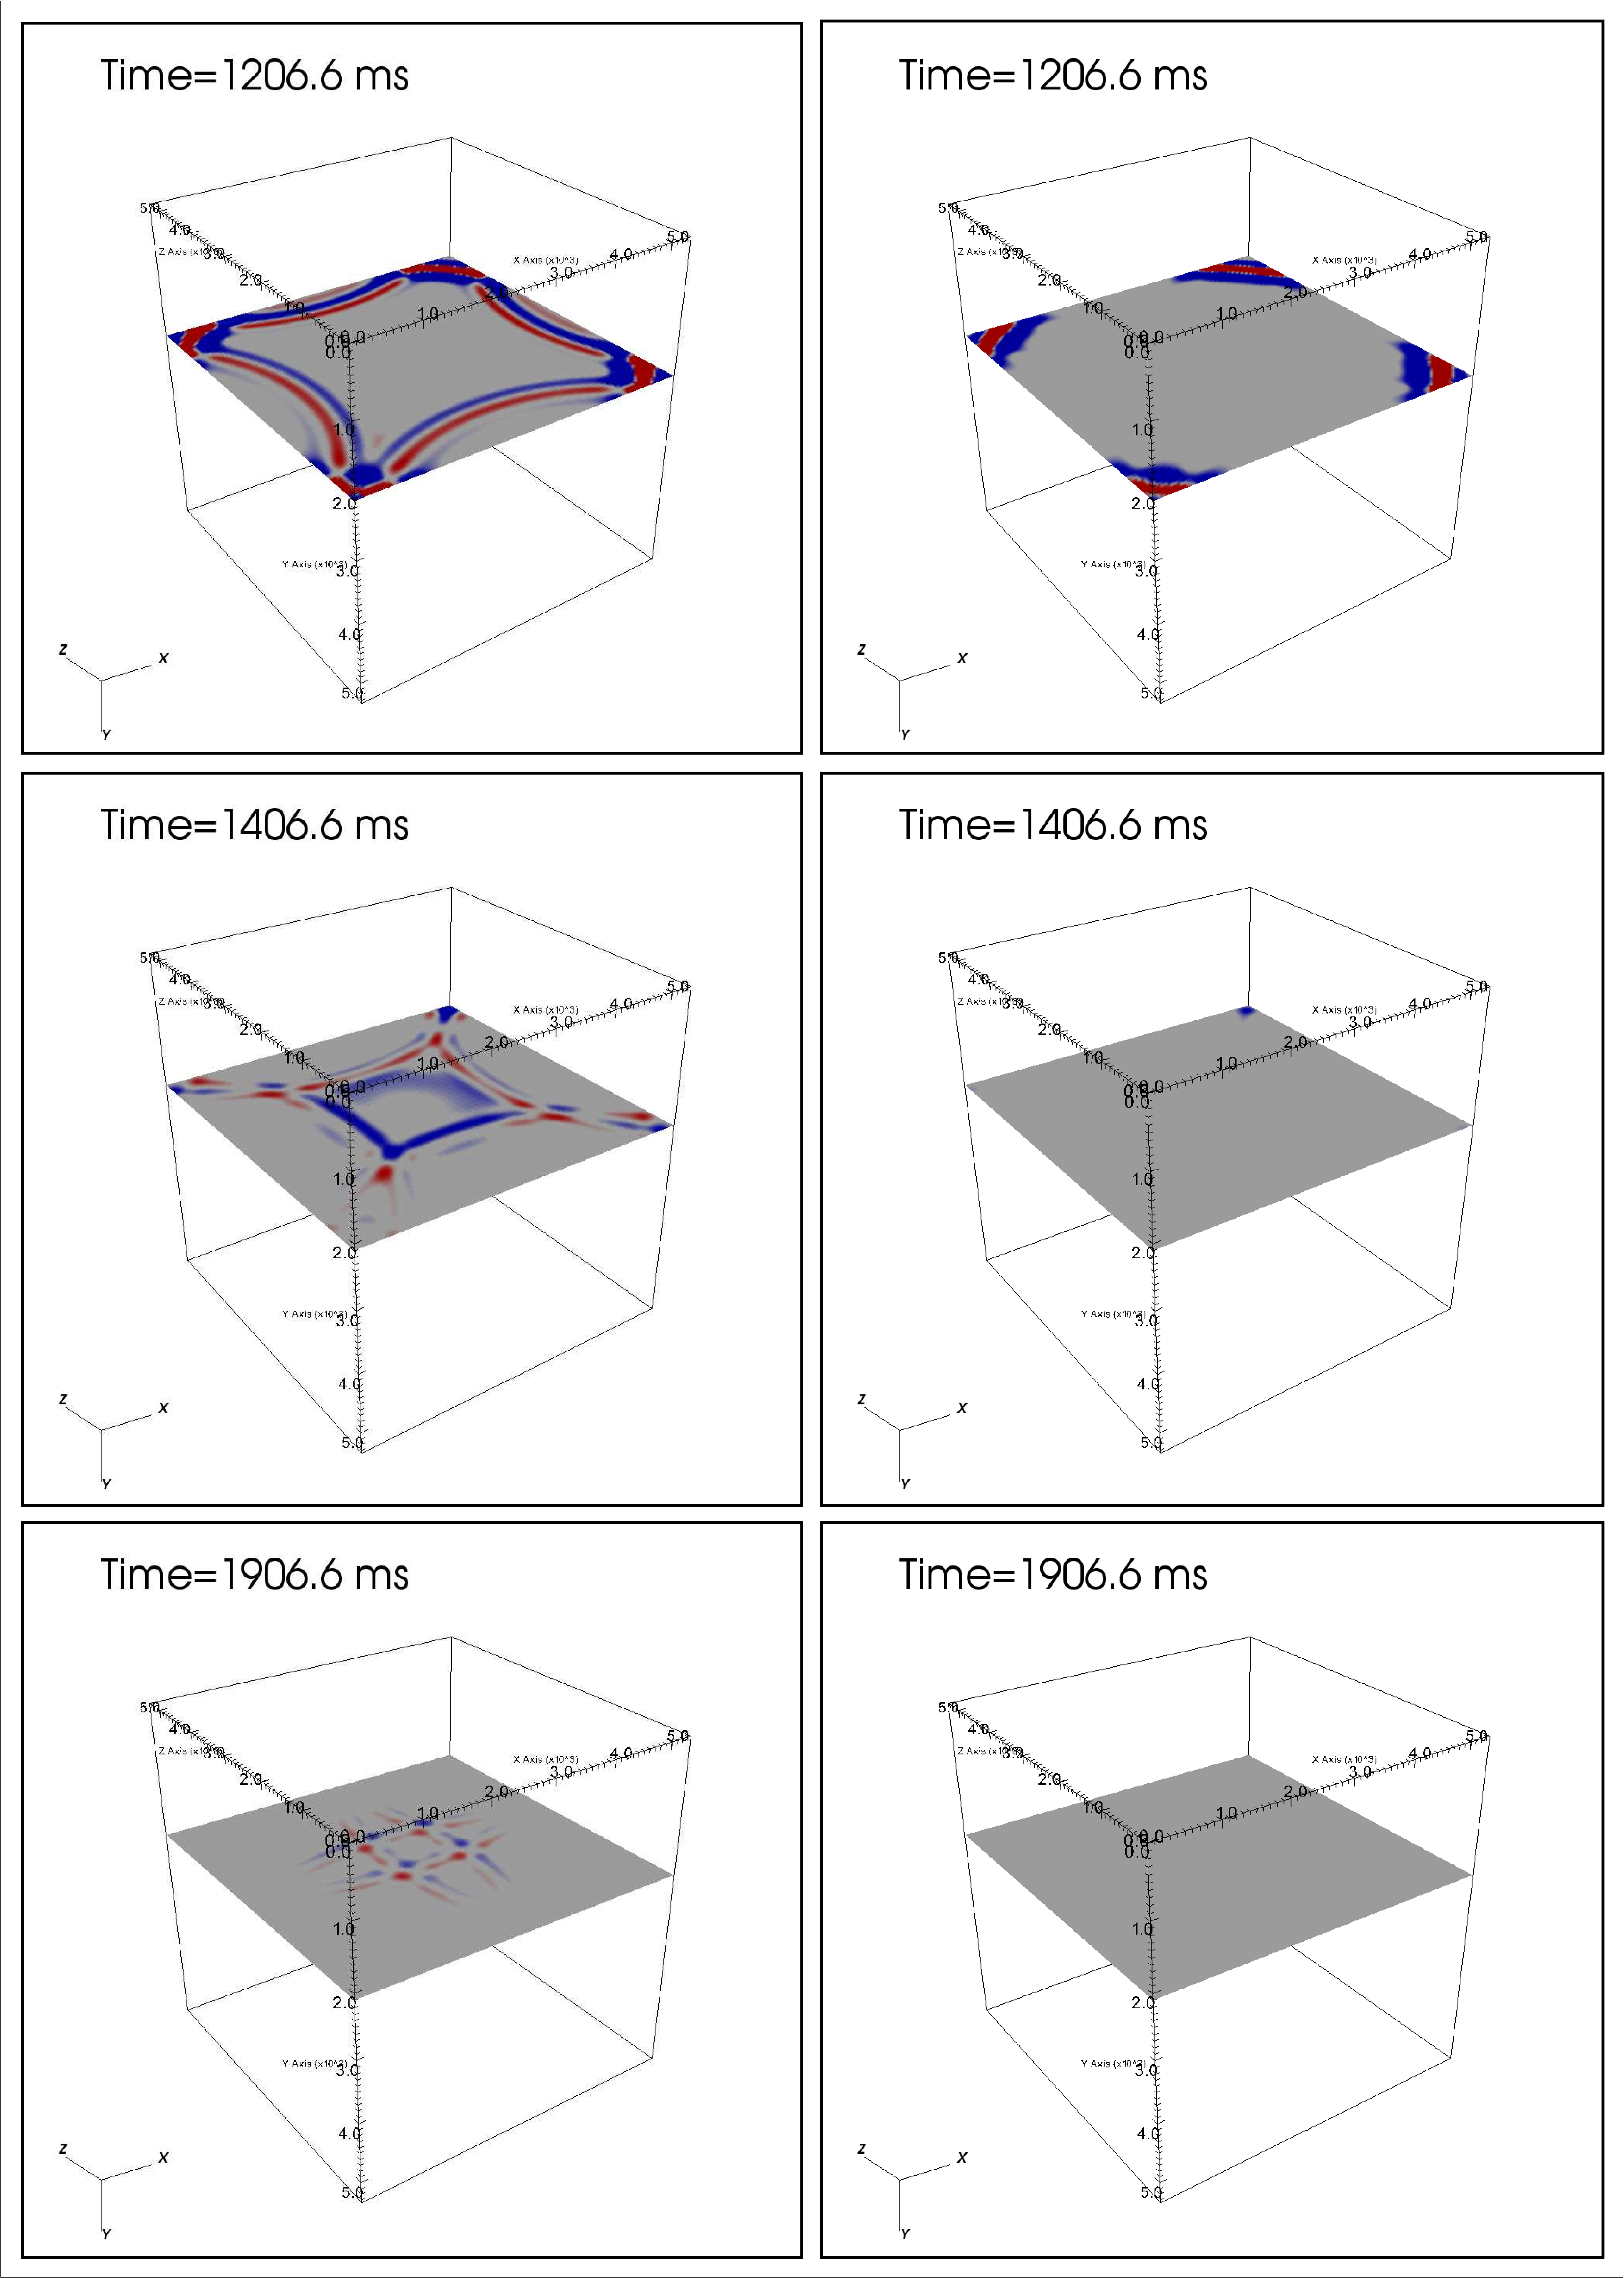
\includegraphics[width=13cm]{figures/ABS_PML_comp_shots.pdf}
\caption{\label{comp_EXP_PML} Comparison between exponential damping (left column) and PML (right column) absorbing boundary conditions for a homogeneous full space model. (\cite{koehn:11})}
\end{center}
\end{figure} 
\end{enumerate} 
\clearpage
\section{Numerical Artefacts and Instabilities}\label{num_instab}
To avoid numerical artefacts and instabilities during a FD modelling run, spatial and temporal sampling conditions for the wavefield 
have to be satisfied. These will be discussed in the following two sections. 
\subsection{Grid Dispersion}\label{grid-dispersion}
The first question when building a FD model is: What is the maximum spatial grid point distance dh, for a correct sampling of the wavefield ? To answer this question we take a look at this simple example: The particle displacement in x-direction is defined by a sine function:
\EQ{grid_disp:1}{\rm{u_x=\sin\biggl(2 \pi \frac{x}{\lambda}\biggr),}}
where $\rm{\lambda}$ denotes the wavelength. When calculating the derivation of this function analytically at $\rm{x=0}$ and setting $\rm{\lambda=1\;m}$ we get:
\EQ{grid_disp:2}{\rm{\frac{d u_x}{d x}\biggl|_{x=0}=\frac{2 \pi}{\lambda} \cos\biggl(2 \pi \frac{x}{\lambda}\biggr)\biggl|_{x=0}=2 \pi.}}
In the next step the derivation is approximated numerically by a staggered 2nd order finite-difference operator:
\EQ{grid_disp:3}{\rm{\frac{d u_x}{d x}\biggl|_{x=0} \approx \frac{u_x(x+\frac{1}{2}\Delta x)-u_x(x-\frac{1}{2}\Delta x)}{\Delta x}\biggl|_{x=0}=\frac{\sin \biggl(\frac{2 \pi (x+\frac{1}{2}dx)}{\lambda} \biggr)-\sin \biggl(\frac{2 \pi (x-\frac{1}{2}dx)}{\lambda} \biggr)}{\Delta x}.}}
Using the Nyquist-Shannon sampling theorem it should be sufficient to sample the wavefield with $\rm{\Delta x = \lambda/2}$. In table \ref{grid_disp.1} the
numerical solutions of eq. \ER{grid_disp:3} and the analytical solution \ER{grid_disp:2} are compared for different sample intervals 
$\rm{\Delta x = \lambda /n}$, where n is the number of gridpoints per wavelength. For the case n=2, which corresponds to the Nyquist-Shannon theorem, the
numerical solution is $\rm{\frac{d u_x}{d x}|_{x=0}=4.0}$, which is not equal with the analytical solution $\rm{2 \pi}$. A refinement of the spatial
sampling of the wavefield results in an improvement of the finite difference solution. For $\rm{n=16}$ the numerical solution is accurate to the second
decimal place. The effect of a sparsly sampled pressure field is illustrated in \FIG{grid_disp_pics} for a homogeneous block model with stress free surfaces. The dimensions of the FD grid are fixed
and the central frequency of the source signal is increased systematically. 
When using a spatial sampling of 16 grid points per minimum wavelength (\FIG{grid_disp_pics}, top) the wavefronts are sharply defined. For $\rm{n=4}$ 
grid points a slight numerical dispersion of the wave occurs (\FIG{grid_disp_pics}, center). This effect is obvious when using the Nyquist criterion ($\rm{n=2}$) 
(\FIG{grid_disp_pics}, bottom). Since the numerical calculated wavefield seem to be dispersive this numerical artefact is called {\bf{grid dispersion}}. 
To avoid the occurence of grid dispersion the following criteria for the spatial grid spacing dh has to be satisfied:
\EQ{grid_disp:4}{\rm{dh \le \frac{\lambda_{min}}{n} = \frac{V_{min}}{n\; f_{max}}.}}
Here $\rm{\lambda_{min}}$ denotes the minimum wavelength, $\rm{V_{min}}$ the minimum velocity in the model and $\rm{f_{max}}$ is the maximum
frequency of the source signal.  
Depending on the accuracy of the used FD operator the parameter n is different.  In table \ref{grid_disp.2} n is listed for different FD operator lengths 
and types (Taylor and Holberg operators). The Holberg coefficients are calculated for a minimum dispersion error of $\rm{0.1\%}$ at $\rm{3 f_{max}}$. For short operators n should be choosen relatively large, so the spatial grid spacing is small, while for longer FD operators n is smaller and the grid spacing can be larger. 
\begin{table}[hbt]
\begin{center}
\begin{tabular}{ccc}\hline \hline
n &  $\rm{\Delta x\; [m]}$ & $\rm{\frac{d v_x}{d x}|_{x=0}\; []}$ \\ \hline 
analytical & - & $\rm{2\pi \approx 6.283}$ \\ 
2 & $\rm{\lambda/2}$ & 4.0 \\ 
4 & $\rm{\lambda/4}$ & 5.657 \\ 
8 & $\rm{\lambda/8}$ & 6.123 \\ 
16 & $\rm{\lambda/16}$ & 6.2429 \\ 
32 & $\rm{\lambda/32}$ & 6.2731\\ \hline \hline
\end{tabular}
\caption{\label{grid_disp.1} Comparison of the analytical solution Eq. \ER{grid_disp:2} with the numerical solution Eq. \ER{grid_disp:3} 
for different grid spacings $\rm{\Delta x = \lambda /n}$.}
\end{center}
\end{table}
 
\begin{table}[hbt]
\begin{center}
\begin{tabular}{ccc}\hline \hline
FDORDER & n (Taylor) & n (Holberg) \\ \hline 
2nd   &   12       &  12         \\
4th   &   8        &  8.32       \\
6th   &   6        &  4.77       \\
8th   &   5        &  3.69       \\ 
10th  &   5        &  3.19       \\
12th  &   4        &  2.91       \\
\hline \hline
\end{tabular}
\caption{\label{grid_disp.2} The number of grid points per minimum wavelength n for different orders (2nd-12th) and types (Taylor and
Holberg) of FD operators. For the Holberg coefficients n is calculated for a minimum dispersion error of $\rm{0.1\%}$ at $\rm{3 f_{max}}$.}
\end{center}
\end{table} 
\clearpage
\begin{figure}[ht]
\begin{center}
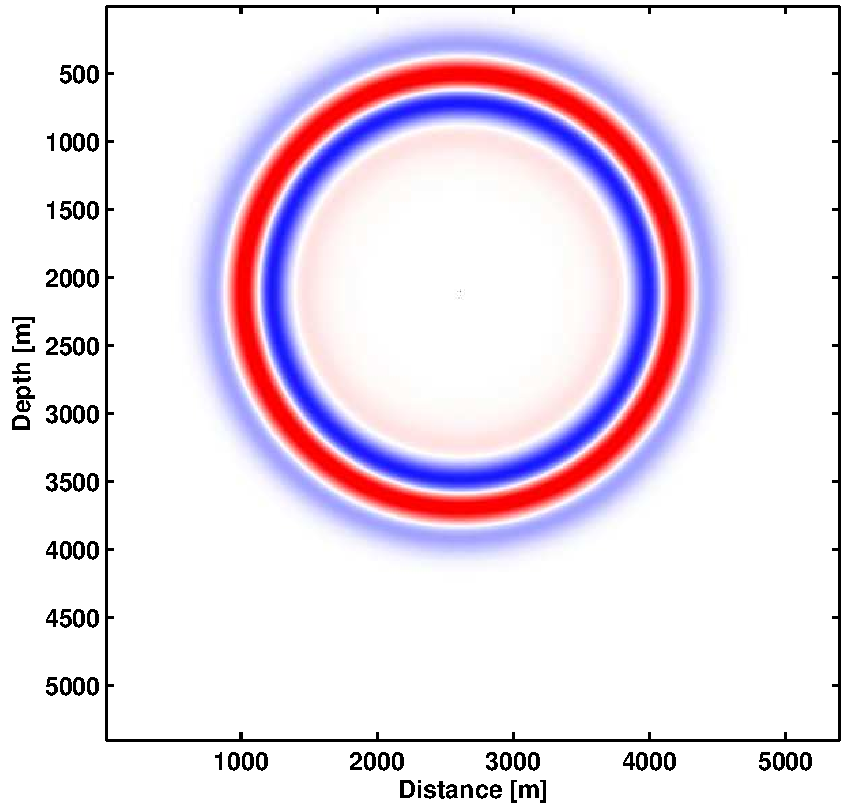
\epsfig{file=figures/homogenous_grid_n_16_5.pdf, width=6 cm}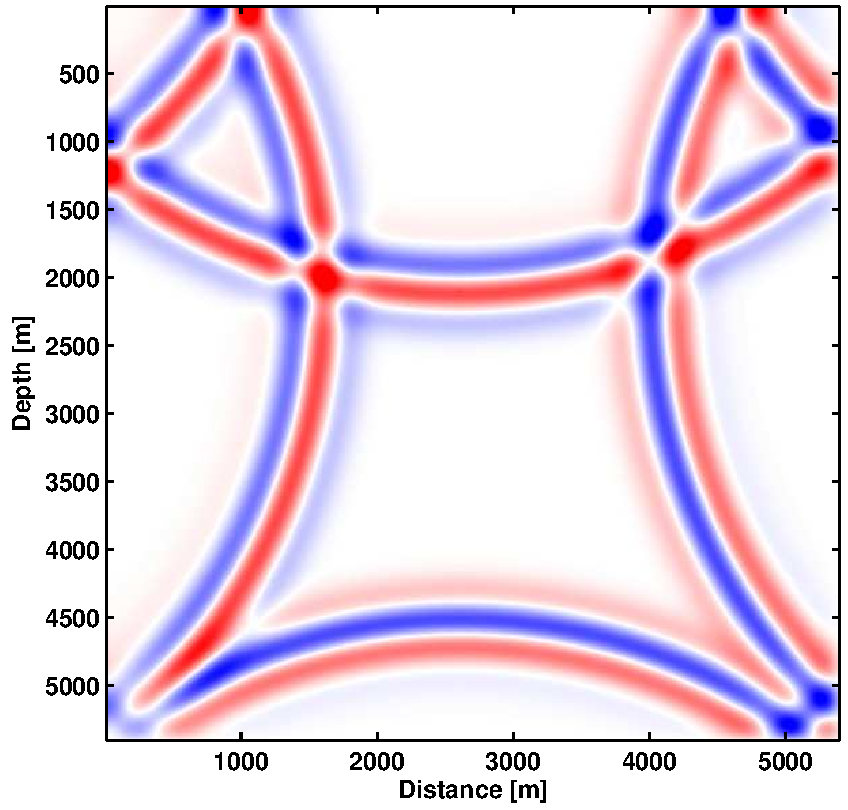
\epsfig{file=figures/homogenous_grid_n_16_10.pdf, width=6 cm}
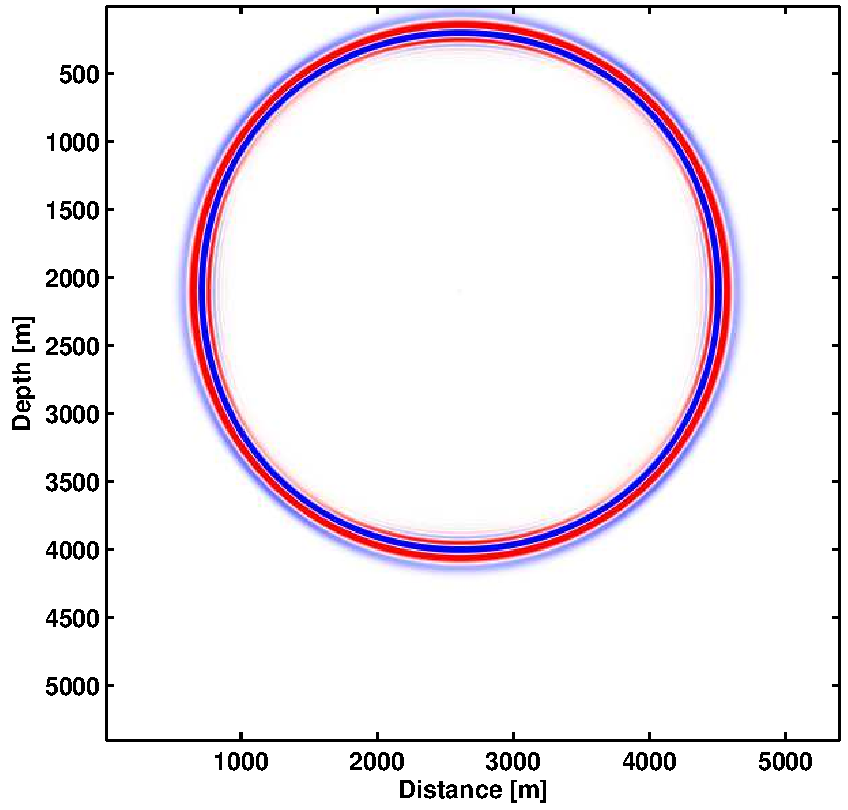
\epsfig{file=figures/homogenous_grid_n_4_5.pdf, width=6 cm}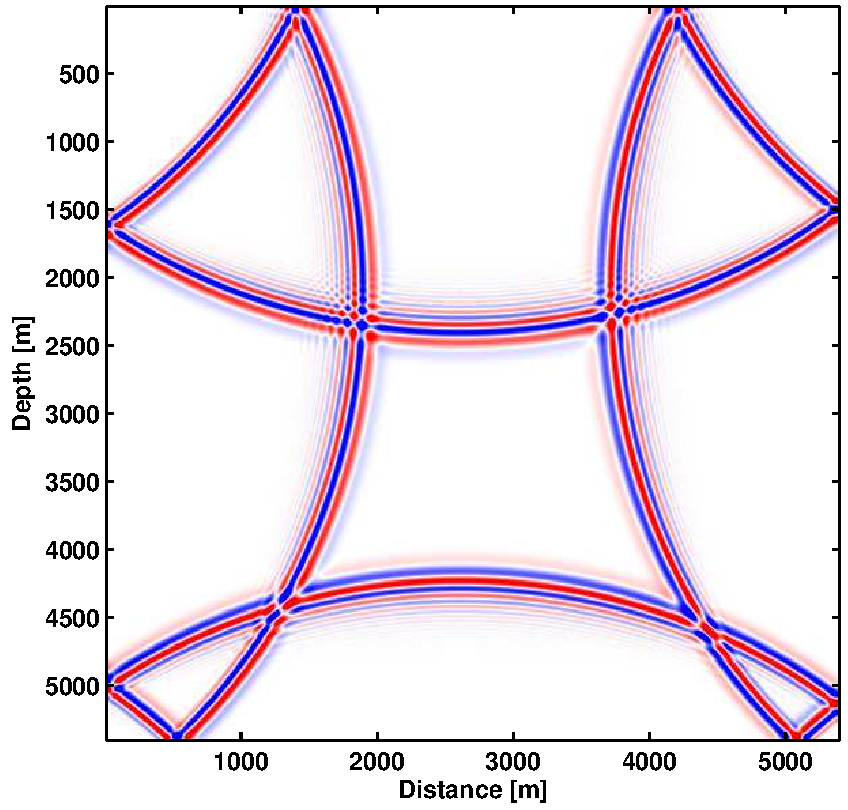
\epsfig{file=figures/homogenous_grid_n_4_10.pdf, width=6 cm}
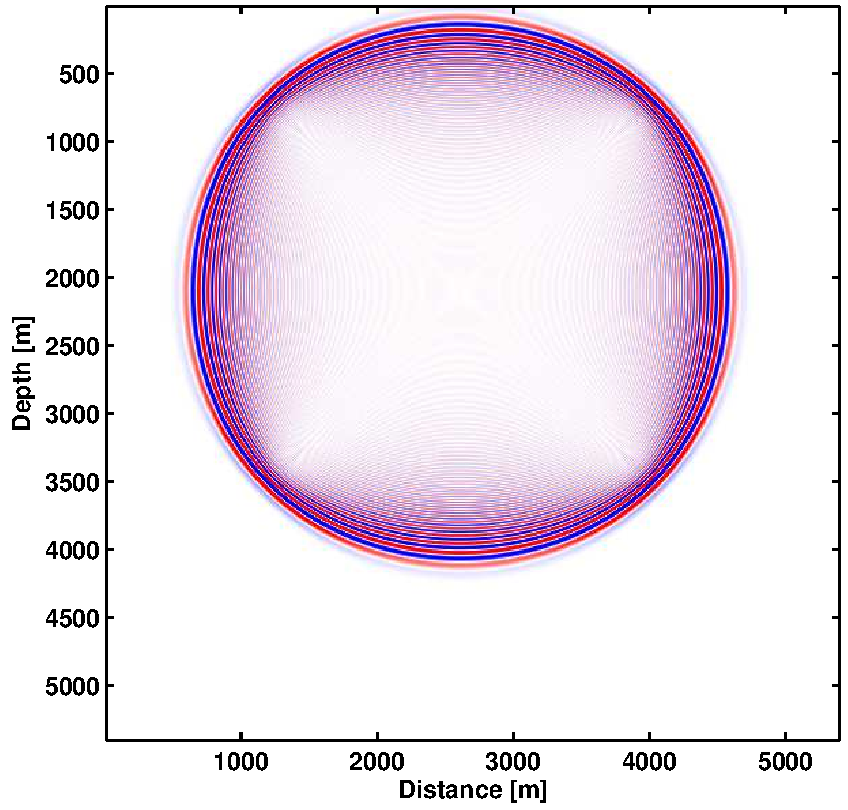
\epsfig{file=figures/homogenous_grid_n_2_5.pdf, width=6 cm}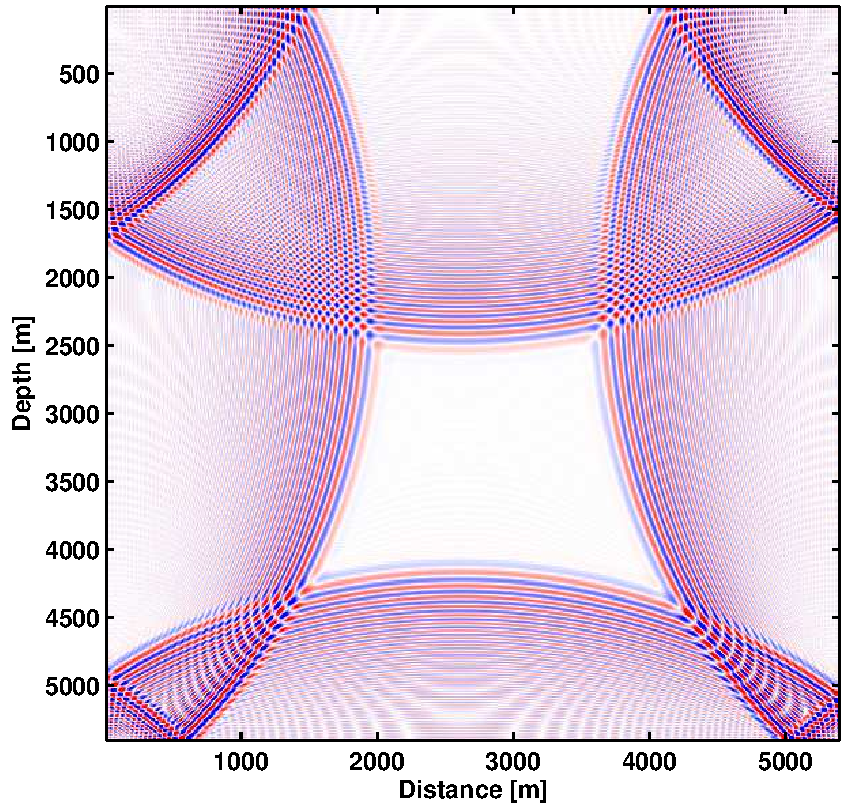
\epsfig{file=figures/homogenous_grid_n_2_10.pdf, width=6 cm}
\caption{\label{grid_disp_pics} The influence of grid dispersion in FD modeling: Spatial sampling of the wavefield using n=16 (top), n=4 (center) and n=2 gridpoints (bottom) per minimum wavelength $\rm{\lambda_{min}}$. (\cite{koehn:11})}
\end{center}
\end{figure}
\clearpage
\subsection{The Courant Instability}\label{courandt}
Beside the spatial, the temporal discretization has to satisfy a sampling criterion to ensure the stability of the FD code. If a 
wave is propagating on a discrete grid, then the timestep $\rm{dt}$ has to be less than the time for the wave to travel between two adjacent grid 
points with grid spacing $\rm{dh}$. For an elastic 2D grid this means mathematically:
\EQ{courandt:1}{\rm{dt \le \frac{dh}{h \sqrt{2} V_{max}},}}
where $\rm{V_{max}}$ is the maximum velocity in the model. The factor h depends on the order of the FD operator and can easily calculated by summing over the weighting coefficients $\rm{\beta_i}$
\EQ{courant:1:1}{\rm{h = \sum_i \beta_i.}}
In table \ref{courant.1} h is listed for different FD operator lengths and types (Taylor and Holberg operators). Criterion \ER{courandt:1} 
is called {\bf{Courant-Friedrichs-Lewy criterion}} (\cite{courant:28}, \cite{courant:67}). \FIG{courandt_pics} shows the evolution of the pressure field when the Courant criterion is violated. After a few time steps the amplitudes are growing to infinity and the calculation becomes unstable.
\begin{table}[hbt]
\begin{center}
\begin{tabular}{ccc}\hline \hline
FDORDER & h (Taylor)      & h (Holberg) \\ \hline 
2nd   &   1.0             &  1.0        \\
4th   &   7/6             &  1.184614   \\
6th   &   149/120         &  1.283482   \\
8th   &   2161/1680       &  1.345927   \\
10th  &   53089/40320     &  1.387660   \\
12th  &   1187803/887040  &  1.417065   \\   
\hline \hline
\end{tabular}
\caption{\label{courant.1} The factor h in the Courant criterion for different orders (2nd-12th) and types (Taylor and Holberg) of FD operators.}
\end{center}
\end{table} 
\clearpage
\begin{figure}[ht]
\begin{center}
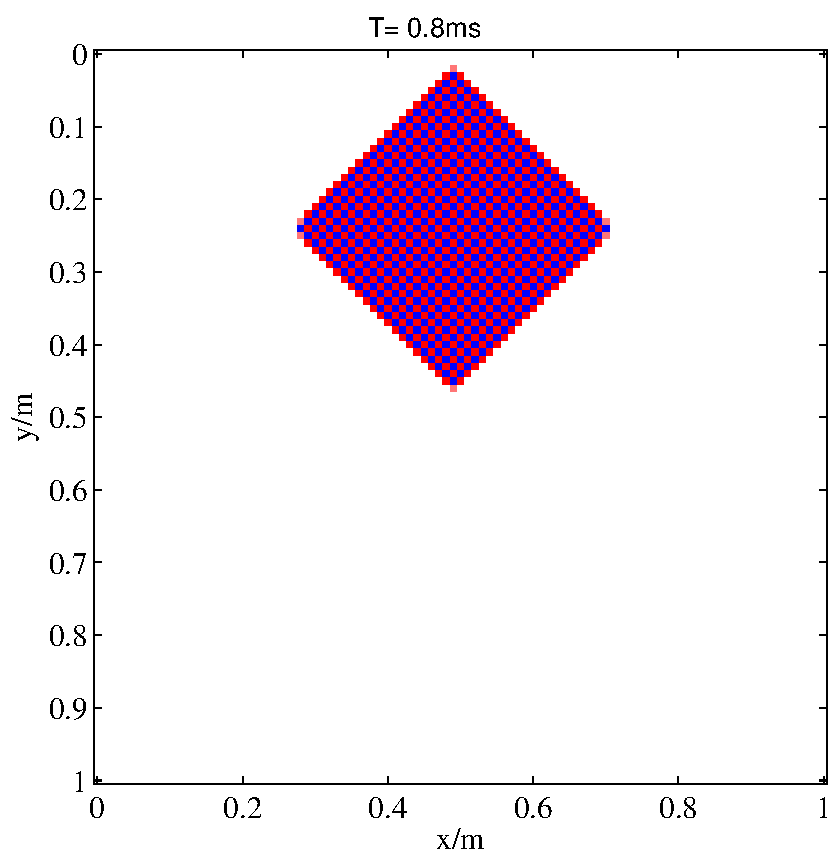
\epsfig{file=figures/courandt_1.pdf, width=7 cm}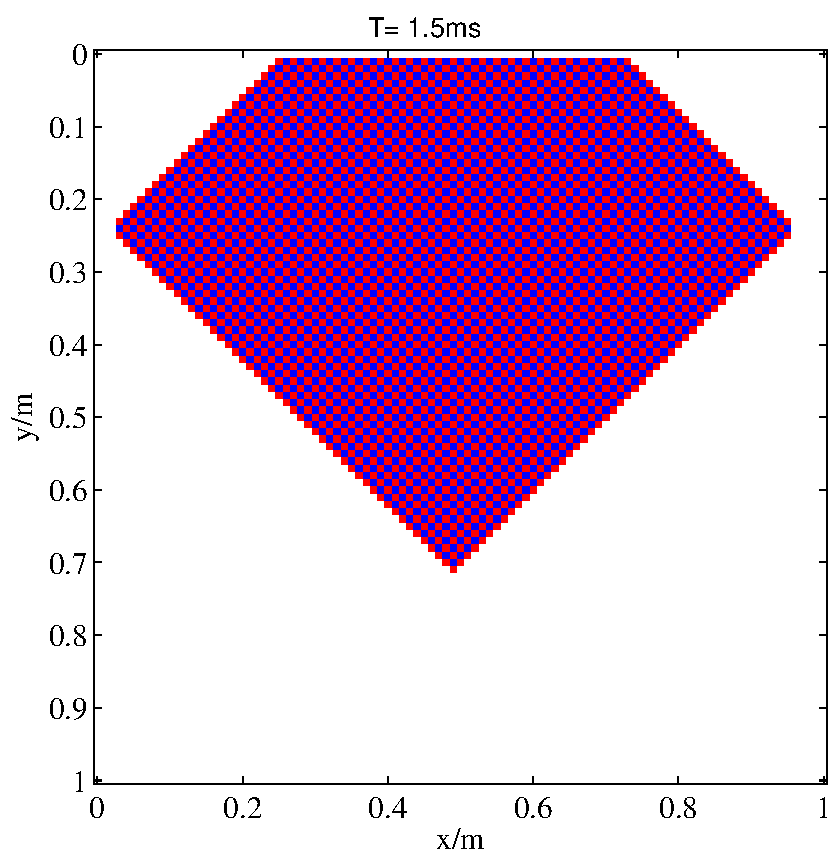
\epsfig{file=figures/courandt_2.pdf, width=7 cm}
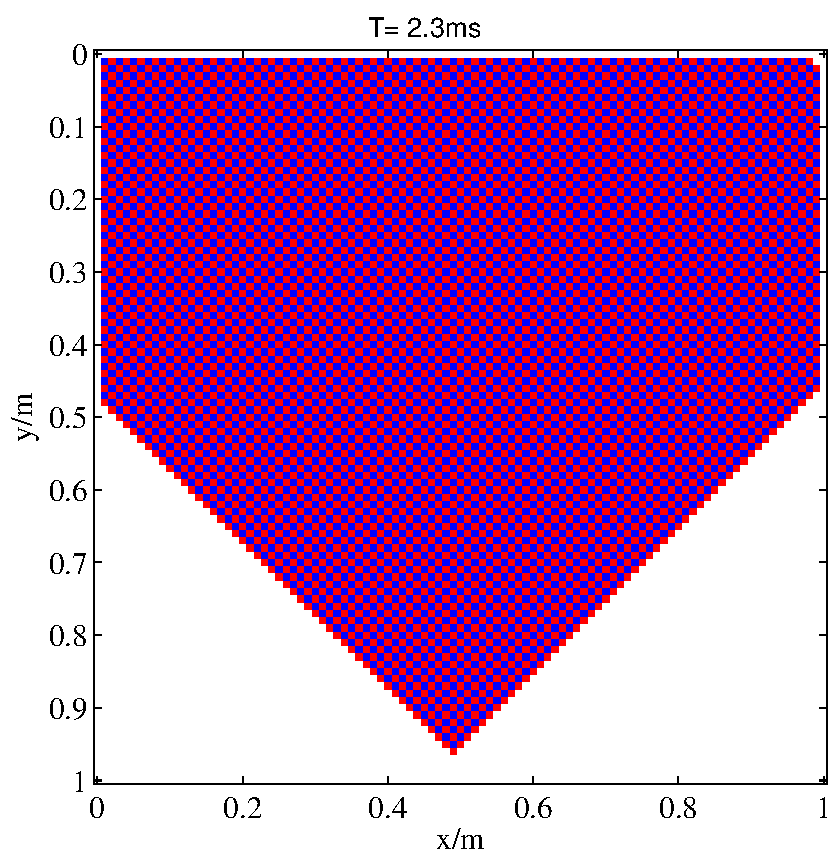
\epsfig{file=figures/courandt_3.pdf, width=7 cm}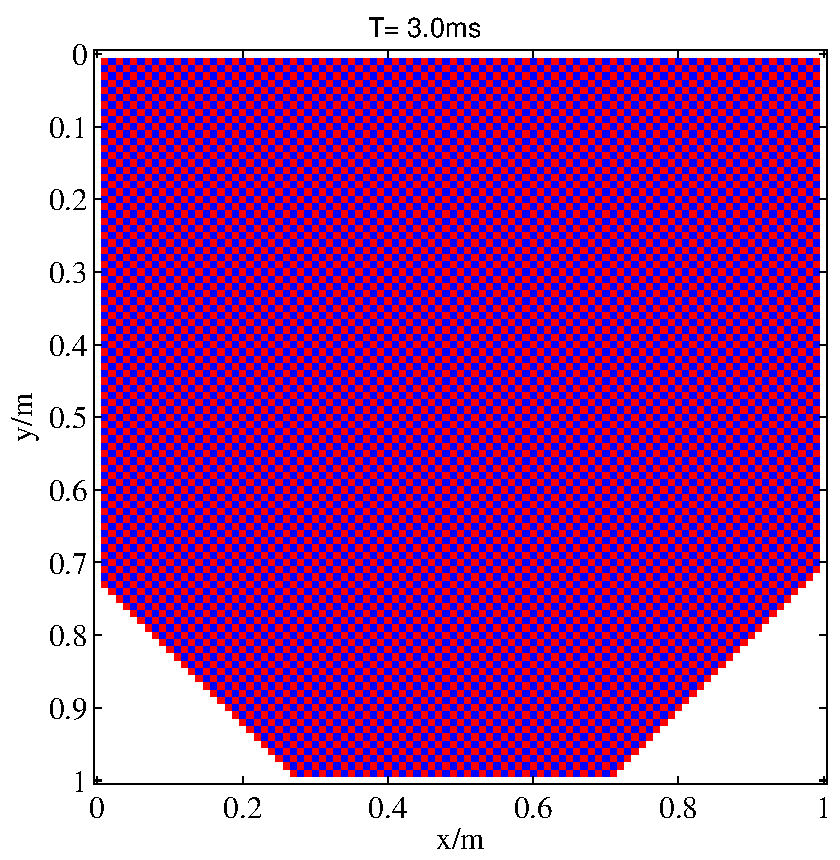
\epsfig{file=figures/courandt_4.pdf, width=7 cm}
\caption{\label{courandt_pics} Temporal evolution of the Courant instability. In the colored areas the wave amplitudes are extremly large. (\cite{koehn:11})}
\end{center}
\end{figure}
\clearpage
